\renewcommand{\theequation}{\theenumi}
\begin{enumerate}[label=\arabic*.,ref=\thesubsection.\theenumi]
\numberwithin{equation}{enumi}

\item Find the tangent at $\myvec{1 \\ 7}$ to the parabola
\begin{equation}
\vec{x}^T\myvec{1 & 0 \\ 0 & 0}\vec{x} + \myvec{0 & -1}\vec{x} + 
6 = 0
\end{equation}
\\
\solution Substituting
\begin{equation}
\vec{p} = \myvec{1 \\ 7}, V = \myvec{1 & 0 \\ 0 & 0}, \vec{u} = \frac{1}{2}\myvec{0 \\ -1}
\end{equation}
%
in \eqref{eq:tangent}, the desired equation is
\begin{multline}
\sbrak{\myvec{ 1 & 7}\myvec{1 & 0 \\ 0 & 0}+\frac{1}{2}\myvec{0 & -1}}\vec{x} 
\\
+ \frac{1}{2}\myvec{ 1 & 7}\myvec{0 \\
-1} 
+6 = 0
\end{multline}
resulting in
\begin{equation}
\myvec{ 2 & -1}\vec{x} 
 = -5
\label{eq:tangent_eg}
\end{equation}
\item The line in \eqref{eq:tangent_eg}
touches the circle
\begin{equation}
\vec{x}^T\vec{x} + 4 \myvec{4 & 3}\vec{x} + c = 0
\label{eq:circle_eg}
\end{equation}
Find $c$.
\\
\solution Comparing \eqref{eq:quad_form} and \eqref{eq:circle_eg},
\begin{align}
\begin{split}
V &= I,
\\
\vec{u} &= 2 \myvec{4 \\ 3}
\end{split}
\end{align}
%
Comparing \eqref{eq:tangent} and \eqref{eq:tangent_eg},
\begin{align}
\vec{p}+2 \myvec{4 \\ 3} &= \myvec{2 \\ -1}
\\
\implies \vec{p} &= -\myvec{6 \\ 7}
%\label{eq:tangent}
\end{align}
%
and
\begin{align}
c +\vec{p}^T\vec{u}&= 5
\\
\implies c &= 5+2\myvec{6 & 7}  \myvec{4 \\ 3}
\\
 &= 95
%\label{eq:tangent}
\end{align}
%
\item Summarize all the above computations through a Python script and plot 
the parabola, tangent and circle.
\\
\solution The following code generates Fig. \ref{fig:parab}.
\begin{lstlisting}
wget 
codes/2d/parab.py
\end{lstlisting}
\begin{figure}[!ht]
\centering
\includegraphics[width=\columnwidth]{./conics/figs/parab.eps}
\caption{}
\label{fig:parab}
\end{figure}

\end{enumerate}
%

